\documentclass[tikz,border=5mm]{standalone}
\begin{document}
	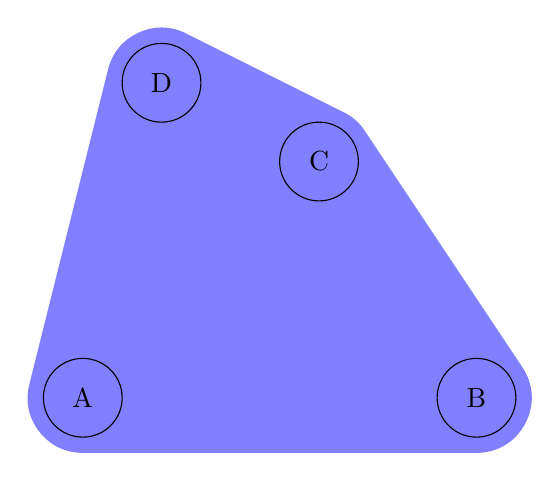
\begin{tikzpicture}
		\tikzstyle{n}=[draw,circle,minimum size=10mm];
		\path 
		(0,0) coordinate (A)
		(5,0) coordinate (B)
		(3,3) coordinate (C)
		(1,4) coordinate (D);
		\path[draw=blue!50,fill=blue!50,line width=1.4cm,line cap=round,line join=round]
		(A)--(B)--(C)--(D)--cycle 
		(A)--(C) (B)--(D);
		\path 
		(A) node[n]{A}
		(B) node[n]{B}
		(C) node[n]{C}
		(D) node[n]{D};
	\end{tikzpicture}
	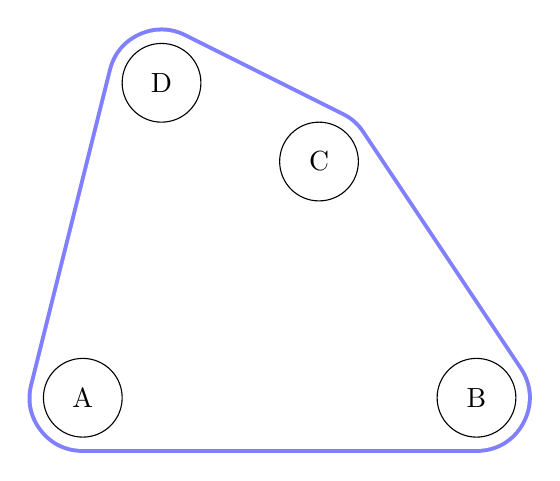
\begin{tikzpicture}
		\tikzstyle{n}=[draw,circle,minimum size=10mm];
		\path 
		(0,0) coordinate (A)
		(5,0) coordinate (B)
		(3,3) coordinate (C)
		(1,4) coordinate (D);
		\path[fill=blue!50,draw=blue!50,line width=1.4cm,line cap=round,line join=round]
		(A)--(B)--(C)--(D)--cycle 
		(A)--(C) (B)--(D);
		\path[fill=white,draw=white,line width=1.3cm,line cap=round,line join=round]
		(A)--(B)--(C)--(D)--cycle 
		(A)--(C) (B)--(D);
		\path 
		(A) node[n]{A}
		(B) node[n]{B}
		(C) node[n]{C}
		(D) node[n]{D};
	\end{tikzpicture}
\end{document}